\chapter{Introduction}
\label{ch:intro}

\section{Overview}
\label{sec:overview}

The Mu2e Raw Data Mover (RDM) System is an element of Mu2e Data Processing
and Computing (DPC)~\cite{DPC}, an L2 project within Mu2e Experiment Operations Plan~\cite{PEOP}.
Its purpose is to move data
that is produced by the online system to long term storage;
for most data, the long term storage will be files on tape in the computer center
but, for some data, it will be in one of the offline databases.
Some data may also reside transiently in disk files in the computer center so that
it is readily available for the follow-on data processing steps.

The full list of computing functions provided by the RDM is:
\begin{enumerate}
\item Move data from the online disk buffer to long term storage.
\item Update the file catalog to include meta-data and file location(s).
\item Any splitting/joining or other reshaping of files that is needed to match the needs of downstream data processing.
\item Manage the free space in the online disk buffer.
\item Manage the free space in the parts of dCache that are critical to data taking.
\item Copy/mirror subsets of the online databases to the offline databases.
\item Copy miscellaneous other files, such as the output of the online Data Quality Monitoring (DQM) system, to long term storage.
\item Provide tools to manage and monitor the RDM system.
\item If needed, inform the follow-on workflows when work is ready for them to do.
\end{enumerate}


%The operation and maintenance of the Mu2e building router and the network between the Mu2e Hall and the computer center
%is the responsibility of the Fermilab Core Computing Division (CCD).
%The DPS has the responsibility to be the interface between Mu2e and CCD regarding this network.
%Details of this responsbility are in Section~\fixme{reference the appropriate section}.

The remainder of Chapter~\ref{ch:intro} will describe some conventions used in this document and
state some prerequisites that will be needed to understand it.
Chapter~\ref{ch:SelectedDetails}  of will describe a view of the
Mu2e Trigger and Data Acquisition system (TDAQ) as seen from the RDM perspective;
it will also describe some elements of the downstream data processing as seen
from the RDM perspective.
Chapter~\ref{ch:DataStreamsAndFileStreams} will define the ideas of data streams and file streams.
Chapter~\ref{ch:data_streams} will give a strawman list of data streams.
Chapter~\ref{ch:file_streams} will give a strawman list of file streams.
Chapter~\ref{ch:requirements} states the requirements for the RDM system.
Chapter~\ref{ch:questions} lists some questions that will need to answered when designing the system.
Chapter~\ref{ch:RiskRegistry} describes risks that are known at this time.
The document includes several appendices that provide some details outside of the main line
of this document.

%The cartoon picture is that TDAQ writes files to a disk buffer and RDM drains the disk buffer.
%However, there are about 30 data streams, some tightly coupled to each
%other, some loosely coupled to the others and others independent of the others.
%The data streams will be grouped into a smaller number of files.


The RDM owns no hardware.  It uses hardware that is owned and maintained
by the Mu2e TDAQ group,
by the Fermilab Scientific Computing Division (SCD)
and by the Fermilab Core Computing Division (CCD).
The only M\&S items within RDM are to pay CCD for maintenance on the Mu2e building router,
and for end-of-service-life replacement of that router;
see Appendix~\ref{app:RouterAndNetwork} for details.

In early planning for the Mu2e DPC, what is now called the RDM was called the Data Logging System.
However that name is too close to two related concepts in the online world:
the {\code artdaq::DataLogger} processes that run on the Data Logger nodes.
To avoid confusion with these other uses of ``Data Logger'',
the name of this task was changed to RDM.

\section{Conventions Used in this Document}
\label{sec:conventions}

In this document the word ``computer center'' is used as a collective noun for the
Feynman Computing Center (FCC) and the Grid Computing Center (GCC).
When it is important to distinguish the two, one of the two will be named explicitly.
This language allows for changes to the computing center infrastructure over the
lifetime of Mu2e.

The DPC is not part of the Mu2e Construction Project but it is part of Mu2e Operations
and Pre-Operations organizations.
In various places, this document refers to ``Mu2e groups'', such as the TDAQ group.
Sometimes this will mean an L2 group within the Mu2e Construction Project and at other
times it will mean a group within the Mu2e Operations or Pre-Operations organizations;
and at other times it will mean a group within the collaboration organization.
Most of the time it will not be important to distinguish between these different meanings
of group; when it is important, it will be stated explicitly.

The phrase ``detector readout electronics'' is intended as collective noun for all elements
up to and including the Read Out Controller (ROC) chips; it does not include
the Data Transfer Controllers (DTC).

This document groups triggers into primary triggers and support triggers.
These ideas are defined in reference~\cite{TriggerSU2020}.



\section{Prerequisites}

This document assumes that the reader has basic familiarity with the \art event processing framework~\cite{ARTWORDPRESS}, including

\begin{enumerate}
\item The ideas of runs and subruns.
\item {\code art::EventID}
\item Event, run and subrun  data products.
\item Run and subrun data product fragments.
\item The notion of an atomic subrun: see appendix~\ref{ch:AtomicSubrunsExtendedDefinition} for a defintion.
\end{enumerate}

It is assumed that the reader knows the roles played within the Mu2e TDAQ by the following:
\begin{description}
\item[OTS DAQ] ``Off-the-shelf DAQ''~\cite{MU2EOTSDAQ}: the software used to provide configuration and top level run-time control of the TDAQ system.
\item[OTS DB] OTS DAQ stores configurations in an instance of a MongoDB database.  This is variously called the ``OTS database'' or the ``Mongo database''.
\item[\artdaq] The software used to move data and to control processes on the DAQ Server and DAQ Data Logger nodes.
\end{description}
Both the OTS DAQ and \artdaq software packages are developed and maintained by Fermilab SCD;
they are used by Mu2e and other experiments. It is not necessary to know details of these packages.

\chapter{External Interfaces}
\label{ch:SelectedDetails}
This Chapter describes a RDM centric view of the external organziations
with which RDM has interfaces.  These include the Mu2e TDAQ system,
the computer center and the follow-on data processing workflows.

\section{Block Diagram}
\label{sec:BlockDiagram}

Figure~\ref{fig:blockdiagram} shows a block diagram of the major elements involved
in the data flow from the experiment hardware to long term storage; it also shows
some of the elements of the offline data processing.
All elements in the left hand dot-dashed box are located in the Mu2e Hall
and, except for the Mu2e building router, are the responsibility of the various Mu2e groups.
All elements in the middle dot-dashed box are located in the computer center
and are the responsibility of SCD; the internal details of the SCD-managed resources
are not shown and the RDM will treat these resources as a interconnected, coherent whole.
The Mu2e building router and the optical fiber that connects that router
to the computer center are the responsibility of CCD;
see Appendix~\ref{app:RouterAndNetwork} for details.
The right hand box shows that Mu2e Offline data processing workflows
will read data from storage in the computer center,
process it,
and write data back to storage computer center.
The first workflow in this chain is Pass1, which will run soon after new files
are registered in the file catalog;
some of the other workflows are shown for completeness.

\begin{figure}[tbp]
\centering
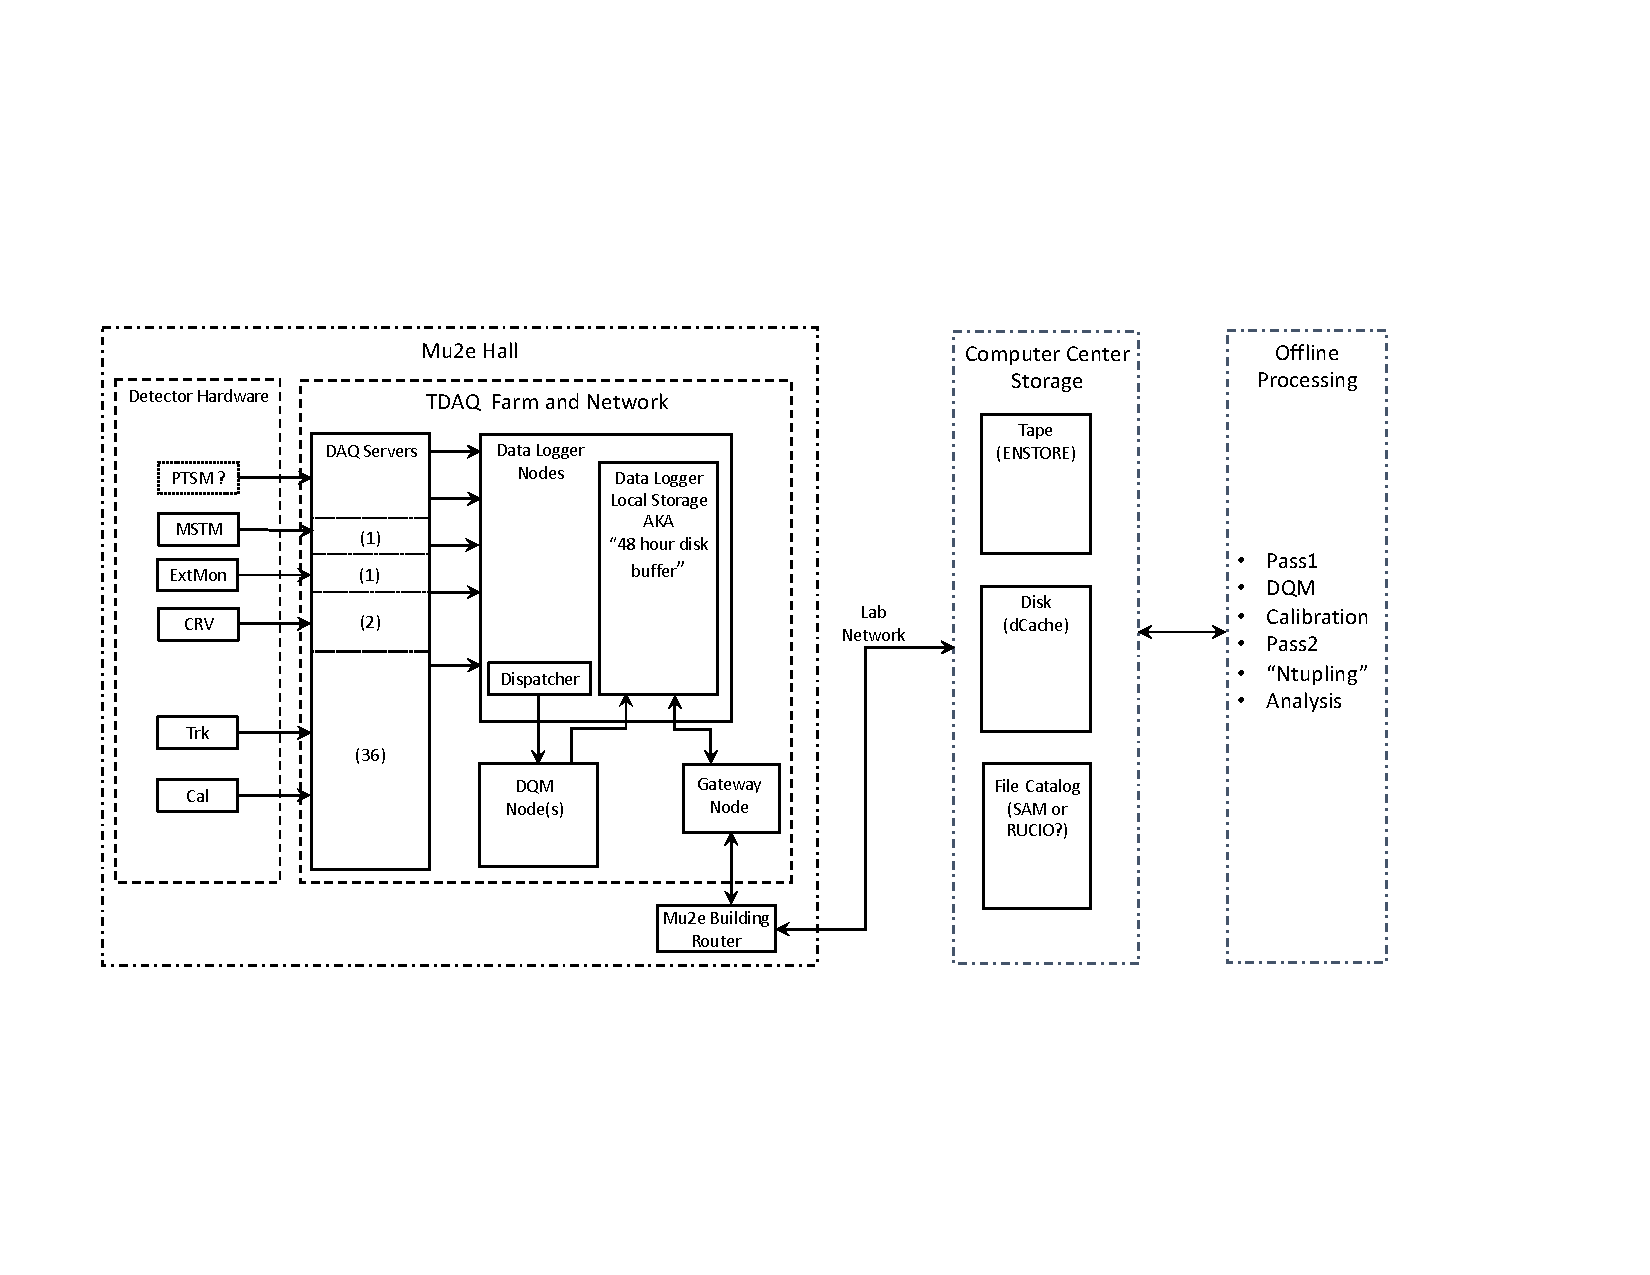
\includegraphics[width=0.9\textwidth]{figures/interface_with_TDAQ.pdf}
\caption[Block diagram of interfaces seen by the Mu2e RDM]{
  Block diagram of the world seen by the Mu2e RDM.
  See the text for a discussion of these elements.}
\label{fig:blockdiagram}
\end{figure}

Data flows from the detectors, through the DAQ system into the TDAQ computer farm.
The five approved detectors are the Tracker (Trk), Calorimeter (Cal), the Cosmic Ray Veto system (CRV),
the Muon Stopping Target Monitor (MSTM) and the downstream Extinction Monitor (ExtMon).
A sixth detector has been proposed, the Production Target Scanning Monitor (PTSM),
which is drawn with a dotted box;
it's primary use is to send rapid feedback to the accelerator control room
and it's not clear what, if any, data it will send through the TDAQ system.
In any event the data volume from that PTSM will be small enough that it will not be
a driver for the RDM.

A cartoon picture of the TDAQ computer farm is that it has 40 DAQ Server nodes
that talk to the detectors, build events and run trigger algorithms on those events.
The design is a dead-timeless streaming DAQ system that has no hardware trigger;
it reads every event from the detector hardware and sends all events to software filters
that run on the DAQ server nodes;
the software makes the trigger decision.
The present design is 20 software filter processes on each of the 40 DAQ server nodes, 800 total.
Events that pass the trigger are forwarded to Data Logger nodes that will write the events
to files in the Data Logger Local Storage (DLLS), a RAID 0 hybrid SSD/HDD array on the bus of the Data Logger nodes.
Appendix~\ref{app:DataLoggerLocalStorage} has the specs for and a discussion about the DLLS.
In earlier DPC related talks and documents the DLLS  was referred to as the ``48 hour disk buffer''.
In addition to the triggered events, a variety of prescaled, untriggered events will pass the
trigger and be handled the same as events that passed the trigger.
Finally, there will be special data streams for calibrations.

The base design is to have a two data logger nodes that receive the data from all DAQ server nodes
and write it to files in the DLLS.
The data logger nodes will write several files, each containing events selected by a different algorithm.
Details can be found in Chapter~\ref{ch:DataStreamsAndFileStreams}.

The Data Logger nodes will also have a process called a ``Dispatcher''
that requests events from the DAQ and forwards them to clients.
The Dispatcher is designed to exert no back pressure on the DAQ
and, therefore, will normally see only a subset of the events.
Two of the clients foreseen for the Dispatcher are an Event Display and
a Data Quality Monitoring (DQM) system,
which will produce histograms, timelines etc that can be viewed in real time.
Periodically the DQM system will write its histograms, log files etc to
files in the data logger local storage.  One of the jobs of the RDM will be
to move these files to long term storage.

All of the computing resources in the TDAQ farm are on a private subnet
and cannot been seen from the lab network.  Access in and out
of the private subnet will be via a gateway node that is connected to
both the private subnet and the lab network.
Purchasing and maintaining the gateway node is the responsibility of the TDAQ group.

When the Mu2e Hall was built and provisioned, CCD personnel installed a dual router
and connected it to the lab optical fiber network.
RDM will move data from the Mu2e Hall
to the computer center using this router and the lab optical fiber network.
The router is standard item that CCD uses in many places and it stocks spares.
CCD is responsible for the maintenance of both the router and the network.
See Appendix~\ref{app:RouterAndNetwork} for the
specs for the router and details of the arrangement with with CCD,
including costs that must be paid by Mu2e to CCD for this service.


For the foreseeable future Mu2e expects that the disk and tape services provided
by SCD will be dCache and ENSTORE.
At this writing Mu2e is using SAM as the file catalog system for files produced
by simulations, tests stands and Vertical Slice Tests (VST).
SCD plans to phase out SAM and replace it with a more modern system, RUCIO\cite{RUCIOHome};
RUCIO is already in use by CMS and by DUNE for Proto-DUNE Single Phase data.
It is likely that SAM will be phased out during the lifetime of Mu2e.
One of the questions to ask in the design of the RDM is
when to make the transition to RUCIO.

\section{The EventWindowTag and the EventMode}
\label{sec:EWTagAndEventMode}

The heart of the TDAQ system is the Command Fan-Out (CFO) that delivers
configuration information and timing signals to all elements of the DAQ.
The inputs to the CFO are the RF0 signal from the accelerator
and a Run Plan that comes from Mu2e DAQ configuration.
Just prior to the start of each event,
the CFO distributes a 16-byte heartbeat packet that describes the upcoming event~\cite{PacketProtocols};
among other things, this contains the EventWindowTag (EWT) and EventMode fields,
both of which will be discussed below.

An event window is defined as time interval during which the DAQ collects data for one event.
Each event window is identified by a 48 bit integer field in the heartbeat packet, called
the Event Window Tag (EWT);
the EWT will be monotonically increasing throughout the Mu2e experiment and
enough bits have been reserved for it to produce unique identifiers for all
events over a many-year run.
The CFO is responsible for incrementing the EWT and putting the correct value into
the heartbeat packet for each event.
The detector readout electronics label information from their subsystem with the EWT.
The event builders use the EWT as the key for event building.

The Mu2e detector can operate in many modes, two of which,
on-spill and off-spill, will be discussed in the next section.
In addition there will be many calibration modes.
All elements of the TDAQ have pre-programmed operations defined for each mode.
When the CFO creates the heartbeat packet for each event,
it sets a 4 byte EventMode (EM) field
that tells the TDAQ system in which mode to operate for the upcoming event.

\section{On-Spill, Off-Spill and Near-Spill}

This section defines the concepts of on-spill, off-spill and near-spill running.

It is expected that, for most of it's running time,
Mu2e will the Fermilab Main Injector with a neutrino experiment,
first, with NOvA and, later, with DUNE.
To keep this document easier to read it will discuss sharing with NOvA but sharing with DUNE is implied.
The change from NOvA to DUNE may change details
but will not materially change the requirements of the RDM.

Sharing with NOvA drives the repeating cycle of Mu2e operations, a Main Injector (MI) cycle of
21 Booster (BO) cycles.
The duration of one Booster cycle is 1/15~s,
making the duration of one MI cycle 1.4~s.
Figure~\ref{fig:beamMacroStructure} shows a cartoon of the MI cycle.
From the Mu2e point of view, the cycle starts with a series of 8 slow spills
from the Delivery Ring (DR) to the Mu2e production target;
within each spill, proton pulses arrive at Mu2e every 1695~ns;
the duration of a spill is nominally 25,438 pulses, about 43.1~ms.
There is a gap of about 5~ms between spills.
The eighth spill is followed by a period of about 1020~ms,
during which no proton pulses arrive at Mu2e;
during this time, beam is delivered to NOvA
and beam is prepared for the next 8 spills to Mu2e.
Then the cycle repeats.

\begin{figure}[tbp]
\centering
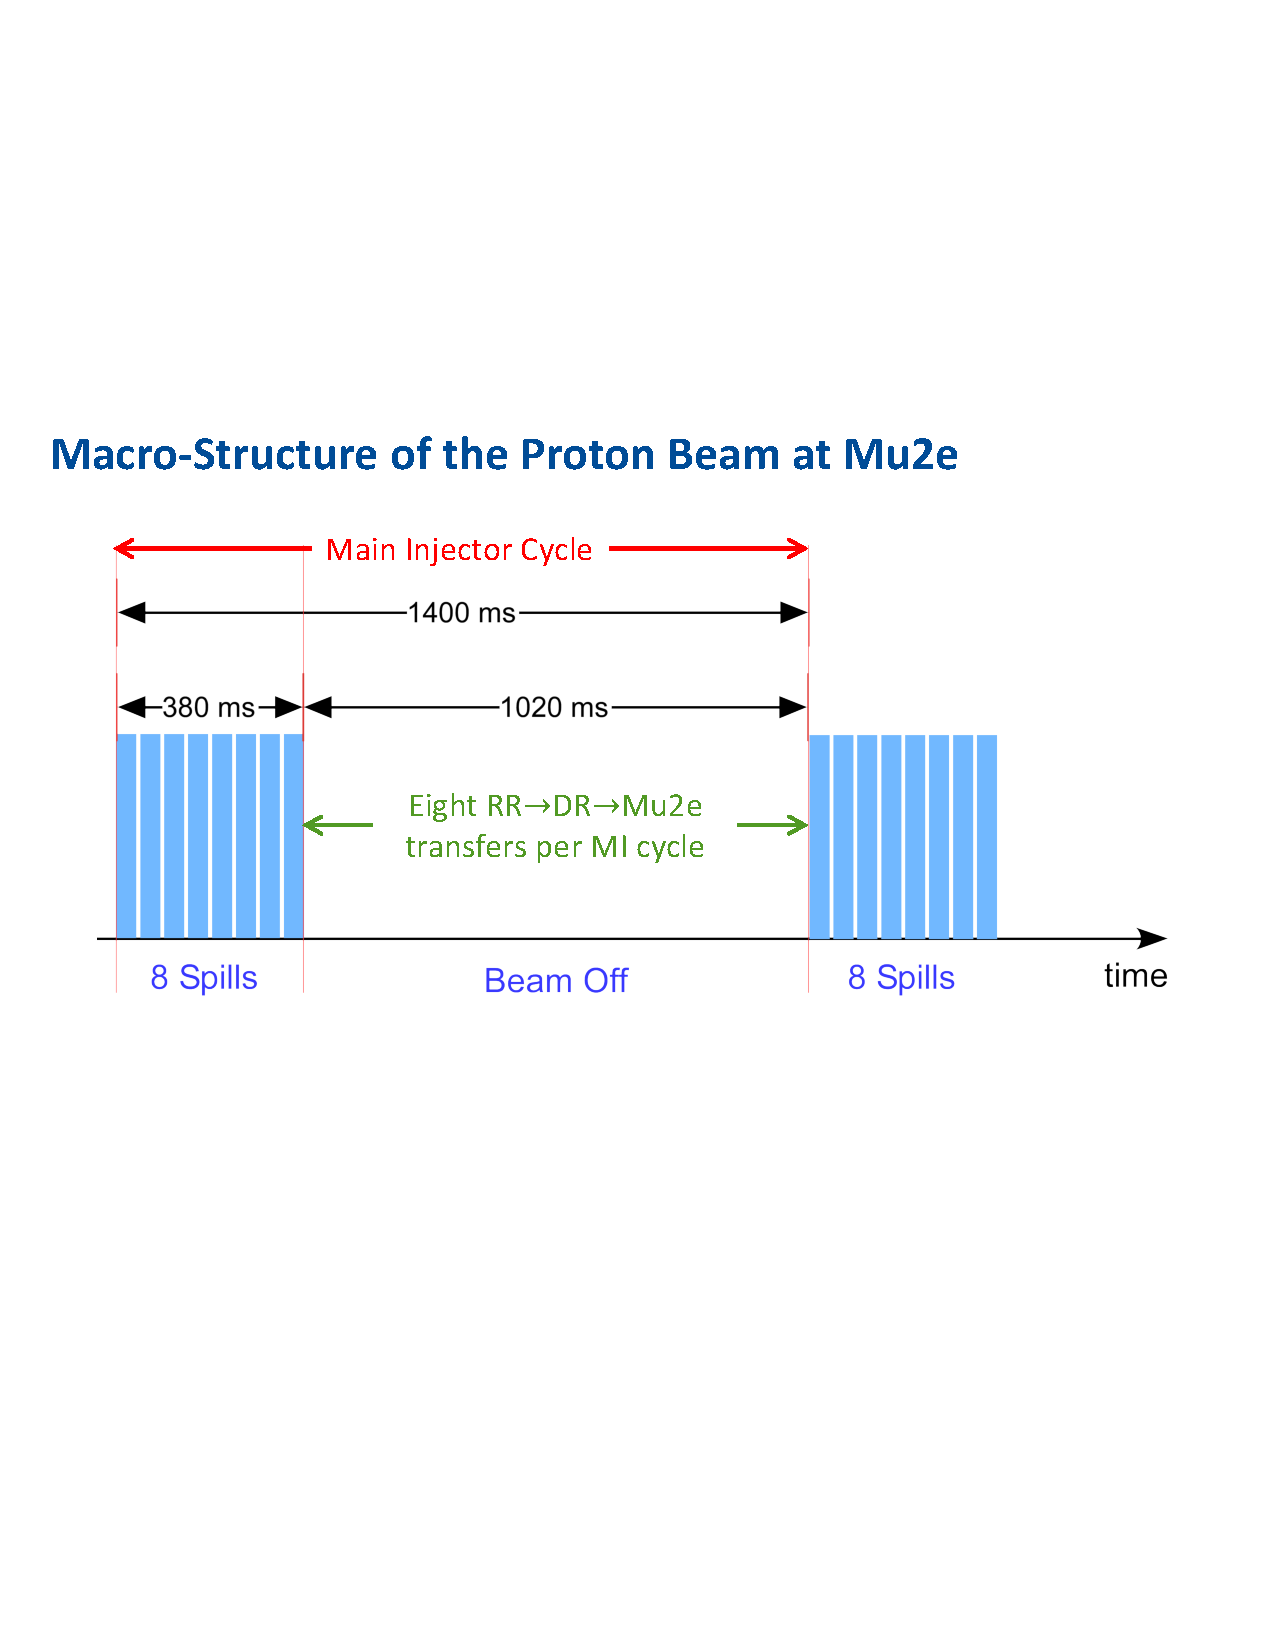
\includegraphics[width=0.9\textwidth]{figures/ProtonBeamLongitudinalStructure2019-01-10_page6.pdf}
\caption[Macro Structure of the Proton Beam at Mu2e]{
  Macro Structure of the proton beam at Mu2e, taken from page~6 of
  the file ``Proton Beam Longitudinal Structure (.pdf)'' from
  Reference~\protect{\cite{beamTiming}}.  The figure is described in the text.}
\label{fig:beamMacroStructure}
\end{figure}

During the spills, Mu2e is running in the on-spill configuration.
During the 1020~ms no-beam period, Mu2e is running in the off-spill configuration.
It has not yet been decided if the 5~ms periods between spills will
be in the on-spill or off-spill configuration
but that does not materially affect the design of the RDM.
Table~\ref{tab:timescales} summarizes the time scales within one MI cycle.
\begin{table}
\begin{center}
\caption[Properties of the Beam-to-Mu2e MI Cycle]{Properties of Beam-to-Mu2e MI Cycle.}
\label{tab:timescales}
\begin{tabular}{ll}\hline
   1/15~s & Period of one Booster cycle \\
   21     & Booster cycles within the MI cycle \\
   1.4~s  & Period of one MI cycle \\
   43.1~ms & Duration of one spill \\
   8       & Number of spills per MI cycle \\
    5~ms   & Duration of the period between two spills \\
   1020~ms & Duration of the off-spill period within one MI cycle \\
   1695~ns & Period of the Delivery Ring and the duration of one on-spill event\\
   100~$\mu$s & Duration of one off-spill event \\
   24.6\%     & Duty factor (total spill time divided by MI cycle duration)\\
   \hline
  \end{tabular}
\end{center}
\end{table}


In the on-spill configuration, one event will have  a duration of 1695~ns
and it records the information associated with one proton pulse.
The trigger will be configured to select interesting events associated with the proton pulse
and to prescale non-triggering events in order to study the performance of the trigger.
In the off-spill configuration, one event will have a duration of 100~$\mu$s.
During the off-spill period, Mu2e will trigger on cosmic rays that
pass through the tracker and/or the calorimeter; it will also collect
pedestal data from some of the subsystems; some calibration procedures
may also take place during the off-spill period.

Mu2e expects that the accelerator super-cycle will consist of a
sequence of many of the above MI cycles,
with an occasional other cycle mixed in.
For example, when MTEST is active, there is usually beam delivered to MTEST about once per minute.
When this occurs, Mu2e will have an extended period of off-spill running.

There will also be periods in which the accelerator complex is not delivering
beam to Mu2e for an extended time, minutes, hours, days or weeks.
In some of these periods Mu2e will shutdown to perform maintenance, repairs or upgrades;
in others Mu2e will execute calibration runs;
and in others Mu2e will collect data in off-spill mode for an extended period of time.


The Mu2e TDAQ team have defined a value of the Event Mode that they have named near-spill.
This is to allow for the possibility that some subsystems may want to
configure themselves differently during the transition from on-spill to off-spill.
At this time there are no definite plans to use this mode but it is available if needed.

The design of the Mu2e TDAQ system is that trigger processing lags the incoming events
during the on-spill period and catches up during the off-spill period.  There is
buffering at various places in the TDAQ system to support this.

It's possible that the MI cycle might need to be increased to 22 BO cycles;
should that happen the additional time will be allocated to a longer off-spill period.
This does not significantly change the requirements for the RDM.

Mu2e plans to start operations with a slightly different configuration:
4 spills instead of 8, where each spill has a longer duration than 43.1~ms;
this mode is called ``one bunch'' running or ``Phase~1'' running;
the 8 spill configuration is called ``two bunch'' running or ``Phase~2'' running.
The data volume produced in one bunch running will be about 60\% of that produced
in two bunch running; otherwise the requirements for the two are the same.

There will be times when Mu2e is taking data but NOvA is not.
In such times, the base plan is that Mu2e will continue to take data using the same MI cycle of 21 BO cycles.
There are several technical limitations that prevent Mu2e from reducing the off-spill period
in order to increase the duty factor:
there are radiation safety limits on the average beam power;
the production target will have a reduced lifetime at higher average beam power;
the TDAQ system cannot accommodate a significantly higher event rate because it
uses the off-spill period to catch up on buffered events.

\fixme{Is the following correct: these limitations have some headroom during one bunch running;
  so we could see a shorter MI cycle during one bunch running.}

\section{EventIDs, Runs and Subruns}
\label{sec:TagsIDsRunsSubRuns}


Mu2e uses the \art event processing framework;
the trigger filter processes that run in the trigger farm will each be a separate \art process;
\art will also be used for offline data processing.
In \art, events are uniquely identified by a 3 part identifier called an
{\code art::EventID}; the parts are named run number, subrun number
and event number.

Within the DAQ system, event fragments and fully assembled events
are identified by the Event Window Tag (EWT).
The DAQ system will translate each EWT to an {\code art::EventID}
before events are presented to the \art based software filter processes~\cite{EventLabels}.
The mapping of EWT to  {\code art::EventID} will be unique and
{\code art::EventID}'s will be monotonically increasing with the time
that the event occurred.
The EWT will be recorded as part of the \art data for each event.

The meaning of run and subrun are defined by Mu2e.
All that \art requires is that a subrun contain zero or more
events and that a run contain zero or more subruns.

The current plan is that runs will typically have a duration of a few hours
while subruns will contain an integer number of MI cycles and
have a duration somewhere between 14 seconds and a few minutes.
This means that each subrun will contain both on-spill and
off-spill events.
The transition between subruns will happen during the off-spill period;
this ensures that each on-spill period is contained within a single subrun.

These durations are informed by the following.
Mu2e has designed a conditions management system
in which intervals of validity (IOV) are a specified as a range of subruns;
such a range may either span runs or be contained within a single run.
Therefore subruns must be short enough to follow the most
rapidly changing conditions.  As of this writing it seems
likely that the upper limit for the duration of a subrun will
be driven by considerations of data handling and downstream data processing;
that is, files should be neither too big nor too small for efficient data handling
and Pass1 jobs should be able to process one subrun in, at most, a few hours.

The Mu2e TDAQ has been designed so that subrun transitions will be deadtimeless
but that data taking will pause for a few minutes at run transitions.
At each run transition the TDAQ system will do some house keeping,
including resetting some hardware, reloading some firmware and restarting some processes.
These steps are designed to cure any Single Event Upsets (SEU) in the firmware
and to generally ensure a robust TDAQ system.
Therefore a run should be long enough that the dead time
caused by the run transition is a small fraction of the total run time
but short enough that the resets occur frequently enough
to keep the system robust.

Anomalies that occur during data taking will cause some runs
and subruns to be cut short.
Therefore the RDM must expect some files that are smaller than normal
and even empty files.


\section{Organization of Data by Detector Subsystem }
\label{ssec:dataOrganization}

This section will give an outline of how data from the
various detector subsystems flows from the detector to the DLLS.
This will help explain why the data organization in the DLLS is what it is.
The text in this section refers to Figure~\ref{fig:filesDLLS}.
These descriptions are only high level overviews,
intended to convey enough information to design the RMD and no more.

\fixme{References to the full TDAQ docs.}

\begin{figure}[tbp]
\centering
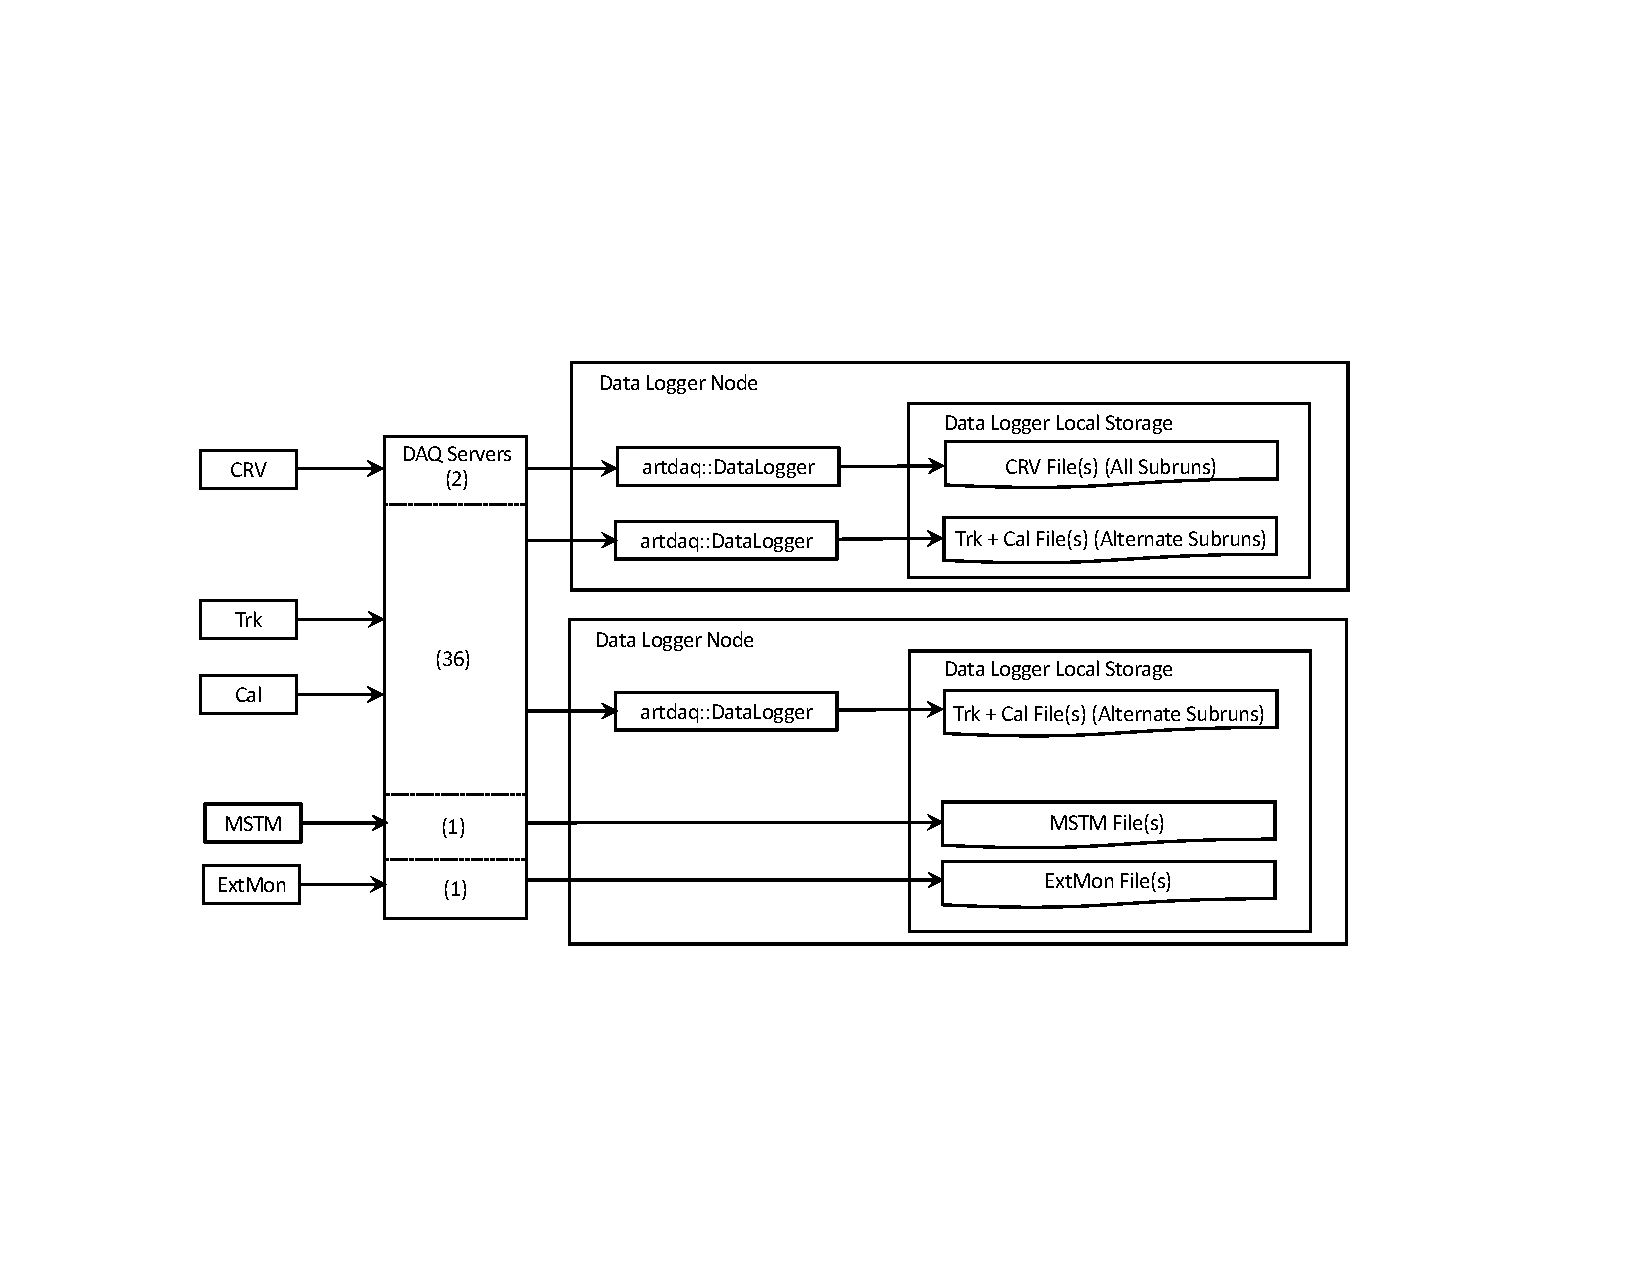
\includegraphics[width=0.9\textwidth]{figures/FilesInDLLS.pdf}
\caption[Files in the DLLS]{
  Files in the Data Logger Local Store; the figure is described in the text.}
\label{fig:filesDLLS}
\end{figure}


\subsection{Tracker and Calorimeter}
\label{ssec:TrkAndCal}

Data flows from the tracker and calorimeter into FPGAs mounted the PCIe bus of 36 of 40 DAQ servers;
these FPGAs are called Data Transfer Controllers (DTC).
All DTCs on these 36 DAQ servers communicate with each other over a high speed switch
and perform event building.
Event building uses only resources on the DTCs and is independent of operations on the host DAQ servers.
The end product of event building is that each DTC contains buffers of complete events held in its own memory;
each event is complete in the sense that it contains all of the data from the tracker and calorimeter
but it does not contain any data from other subsystems.
Every event is present in exactly one buffer and each DTC sees only a small subset of the full event stream.

Once a DTC has a full buffer of events it will transfer that buffer to its host DAQ server;
it does so by transferring it to an {\code artdaq::BoardReader} process.  On most of the
36 DAQ severs there are two DTCs and two {\code artdaq::BoardReader} processes;
on the remaining servers there is one DTC and one {\code artdaq::BoardReader} process.

The trigger filter processes on each DAQ Server are controlled by a process
called an {\code artdaq::EventBuilder}.
This name is historical and reflects the function that it had for earlier experiments in which \artdaq was developed.
For Mu2e, event building will be done in the DTCs and the function of an
{\code artdaq::EventBuilder} process is to receive events from one of
the {\code artdaq::BoardReader} processes and to distribute them to the trigger filter \art processes.

If an {\code artdaq::EventBuilder} has trigger filter processes that are ready for their next event,
and if no events are available from {\code artdaq::BoardReader} process(es) on that server,
then the {\code artdaq::EventBuilder} can fetch event buffers from {\code artdaq::BoardReader} processes
on other DAQ servers.
This allows all 40 DAQ servers to run trigger filter processes even though only 36 of the 40 servers
communicate with the tracker and calorimeter.

The end result is that each event will be seen by exactly one of the trigger filter processes.
Within one trigger filter process there is no guarantee that events within one subrun will arrive in
increasing order of {\code art::EventID}.

\fixme{Is there a guarantee that, within a single process all events from subrun n will be seen before
  any events from subrun n+1?  If so, for personal interest, how is this guaranteed?
  I am thinking of a process running on, the CRV, ExtMon or MSTM servers; these get all of their
  events from BoardReaders on other machines.  I can see that they will usually be in increasing order
  but I don't see a requirement that they be in increasing order.
}

The trigger filters make a trigger decision on each event.
The current design is that about 1 in 400 events will pass the trigger;
this includes all events that pass the primary triggers,
prescaled events that pass the support triggers,
and prescaled events that fail at selected places during trigger processing;
random triggers are included in the last category.
Throughout this document the phrase ``passes the trigger'', without additional modifiers,
refers to all of the above.
The trigger rate is dominated by prescaled support triggers,
which are designed to select events for calibration and monitoring.
Details of the software trigger system, as of May 2021,
are available in reference~\cite{TriggerSU2020}.


Each \art trigger filter process sends events that pass the trigger over a standard ethernet
to one of the two data logger nodes where they are received by an {\code artdaq::DataLogger} process
that writes the events to files in the DLLS.
This process may be configured to write all events to a single file
or to split the events across several files,
for example all on-spill events to one file and all off-spill events to another.
It has yet to be determined exactly how many files will be written
by each {\code artdaq::DataLogger}.

Because different events have very different processing times in the trigger processes,
and because {\code artdaq::EventBuilder} processes can draw events from
any of the {\code artdaq::BoardReader} processes, events will arrive at the
{\code artdaq::DataLogger} out of order.  In particular, early events from subrun N+1
may arrive at the {\code artdaq::DataLogger} before the last event from subrun N.

The TDAQ base design has two Data Logger nodes, each running an
{\code artdaq::DataLogger} process that will receive tracker and calorimeter events.
The plan is to send events from alternate subruns to each of the two.
This allows a clean separation of the event stream into non-overlapping subruns.
Within a each subrun, however, the events may not be in order.

\fixme{If we end up with short subruns, say 10 MI cycles, 14 s, will we need to stripe
  this 3 or 4 wide to survive the longest processing latencies?}

At the big picture level the above story is the same for both on-spill and off-spill running.
There are two important differences in details.
First, the trigger filter processes test the EventMode
and run different algorithms for the two cases;
second, the rate of triggered events
and data volume per triggered event will be much smaller in off-spill events than in on-spill events.


The behavior for other event modes will be discussed elsewhere.
\fixme{Add references}

\subsection{Cosmic Ray Veto}
\label{ssec:CRV}

In on-spill running,
data from the CRV system is read from the detectors and held in buffers in the
readout electronics chain.
When one of the trigger filter processes described in the previous section
decides that an event has triggered,
it sends a message to the CRV system and requests that information from that
event be forwarded to a Data Logger node.
The requested information flows from the readout electronics through 2 two of the 40 DAQ servers
to a third {\code artdaq::DataLogger} process that is running on one of the Data Logger nodes.
This third {\code artdaq::DataLogger} process writes the events to files in the DLLS.
Again, this process may be configured to write all events to a single file
or to split the events across several files,
perhaps on-spill events to one file and off-spill events to another.
The details are to be determined.

\fixme{where are the buffers? ROC? FEB?}

The end result is that each event in the DLLS will be split across two files, one with the
tracker and calorimeter data and one with the CRV data.
One of the questions to be answered when designing the RMD will be to identify
the point in the workflow that these two event fragments will be joined into a single file.
There are insufficient computing resources to do this step in the Mu2e online environment.
Therefore it will have to be done after data has been copied to the computer center.
One of the questions in designing the RDM will be to work with the Pass1 team to
decide if the responsibility for this job is part of the RDM or if it is part of Pass1.

The original design of the TDAQ was the that an {\code artdaq::DataLogger} process
would receive the tracker and calorimeter information for trigger events
and buffer it internally until the CRV information arrived.
After the CRV information arrived,
the {\code artdaq::DataLogger} process would write an event containing information from all 3 subsystems.
Recently the TDAQ team became concerned that this scheme would not work because
the tail to long processing times in the trigger filters would exceed the buffering capacity within
the CRV readout electronics.
Therefore this plan was replaced with the two file solution.


The light sensors for the CRV system are Silicon Photo multipliers (SiPM).
The CRV team have requested that, during off-spill running,
TDAQ acquire as large a sample of SiPM noise as is practical;
they will use this data to study the time dependence of the SiPM pedestals.
This data is sometimes called ``SiPM noise data'' or ``SiPM pedestal data''.

Mu2e will automatically get a small sample of SiPM noise from the off-spill events
that trigger based on tracker and calorimeter data.
However this trigger rate will be only a few Hz, which will not yield enough SiPM noise.
One option is for the trigger filters to prescale off-spill events that fail the trigger
and to do so at a rate that will produce a large enough sample of SiPM noise.
In this case SiPM noise events will include information from the tracker and calorimeter as well,
albeit in separate files.
A second option is for an independent agent within the TDAQ system to trigger the SiPM noise events;
in this case most SiPM noise events will usually not contain tracker and calorimeter information.
The TDAQ team has not yet decided between these options.

\fixme{If the collaboration has a preference, they should make it known.}

\subsection{Extinction Monitor}
\label{ssec:ExtMon}

The Extinction Monitor system sends its data to a single node in the DAQ server farm.
That server will receive the data and write it to one or more files in
the DLLS.  This server will also have trigger filter processes that receive
data from buffers on the 36 servers that talk to the tracker and calorimeter.

\fixme{Understand some more about the mechanics.  Are there {\code artdaq::DataLogger} processes involved.
  How is data transferred to the data logger node?  Eric says no NSF mount because of reliability.  So
  something else.
  }

\subsection{Muon Stopping Target Monitor}
\label{ssec:MSTM}

The Muon Stopping Target Monitor sends its data to a single node in the DAQ server farm.
That server will receive the data and write it to one or more files in
the DLLS.  This server will also have trigger filter processes that receive
data from buffers on the 36 servers that talk to the tracker and calorimeter.

\subsection{Production Target Scanning Monitor}

The principle client for data from the PTSM is the accelerator control room.
At this writing it has not yet been defined if it the PTSM will write any data the the DLLS.
Should that happen it is likely that the pattern will be the same as for the ExtMon
and MSTM.


\chapter{Data Streams and File Streams}
\label{ch:DataStreamsAndFileStreams}

This chapter defines the ideas of ``data streams'' and ``file streams''.
It enumerates the data streams that are anticipated at this time
and it presents a straw man for how these may be grouped into files.

\fixme{Should I use the word ``data set'' instead of ``file stream''?
  I am using a distinct word for now since I want to reserve the word
  of data set for something that is defined using SAM.  Are these
  two ideas identical?
}

A ``data stream'' is a series of events selected by some algorithm;
one attribute of events in a data stream is they all require the same downstream processing.
For example the on-spill and off-spill events are distinct data streams.
The on-spill events will have many trigger lines; one might consider each trigger
line it's own data stream or one might define groups of trigger lines as a data stream.
Another example: the off-spill events will include some events that triggered based on
the tracker or calorimeter and they will also include SiPM noise events.
These are distinct data streams.

A ``file stream'' is a series of files that contain events from one or more data streams.
For example we might decide to bundle all of the on-spill data streams into a single
file stream or we might decide to put some of the on-spill data streams into one file
stream and another set of on-spill data streams into a different file stream.
For example all of the files containing off-spill events might be one file stream;
or maybe we will decide to split the off-spill events in to
the two off-spill data streams into two file streams.

The key point is that data streams are a physics driven idea,
while file streams are choice about how to group data streams for convenience of data handling and downstream processing.

\fixme{We need to address if a given event may be in more than one data stream.
       And we need to address if a given data stream may be in more than one file stream.
}

The design of number of file streams and the grouping of data streams in to file streams
is in progress.
In an ideal world the TDAQ would chose to organize data into file streams that best match the needs
of downstream processing.
This pushes the decision towards more file streams.
However there are overheads associated with each file stream and that may force Mu2e to fewer file streams
than optimal for downstream processing.
If this happens, the DPC organization will need to decide where in the workflow to perform
the reorganization of the data.

% Example
% Keep sections under development
%\IfStrEq{\ISDRAFT}{YES}{
%
%\chapter{A Chapter under development}
%\label{ch:under_development}
%
%This is a chapter still under development.
%It is kept here to illustrate the use of the  ISDRAFT macro.
%
%} % end `ISDRAFT = YES'

\chapter{List of Data Streams}
\label{ch:data_streams}

This chapter lists all of the data streams known at this time.

\section{On-Spill Data Streams}
\label{sec:on_spill_data_streams}

\begin{enumerate}
\item Triggered, Trk+Cal
\item Triggered, CRV
\item Intensity stream
\item ExtMon - 4 data streams
\item MSTM - 4 data streams
\end{enumerate}

\section{Off-Spill Data Streams}
\label{sec:off_spill_data_streams}

\begin{enumerate}
\item Triggered, Trk+Cal
\item Triggered, CRV
\item SiPM Pedestal, CRV
  \item SiPM Pedestal, Trk+Cal (may not exist)
\item ExtMon???
\item MSTM - Will continue to produce the same 4 data streams for at least 10 minutes into an extended shutdown.
\end{enumerate}

\section{Other Data Streams}
\label{sec:Other_data_streams}

\chapter{Strawman for the File Streams}
\label{ch:file_streams}


\chapter{Requirements}
\label{ch:requirements}

This chapter lists requirements for the RDM system.

\begin{enumerate}
\item Move data from DLLS to long term storage in a timely fashion.
  \begin{enumerate}
  \item In normal operations this should be complete within N minutes of the end of data taking for that subrun. \fixme{N=5? 10? 15?}.
  \item 95\% of the time, Pass1 for a subrun must be complete within 6 hours of the end of data taking for that subrun.
  \item The TDAQ will produce some files that need to travel in pairs, for example Trk+Cal on-spill file and CRV on-spill file.
    Prioritize data handling to move these together.
  \item When dCache is not available, data will pile up in the DLLS.  When service is restored prioritize data handling of the backlog
    so that the highest priority files are copied first.
  \end{enumerate}
\item Most data sets should be written to a file family that makes two copies on tape in physically separate locations.
  There may be some data sets for which a single copy is adequate.
  Work with the collaboration to decide which data set falls into which category.
\item Update the file catalog to provide meta-data and locations for all new files.
\item Copy/mirror information in the various online databases to the appropriate offline databases.
  \begin{enumerate}
  \item Prioritize any information that is needed for Pass1; an example is that Pass1 may want the conditions information
    used by the trigger filter processes.
  \end{enumerate}
\item Copy other files from online disks to long term storage; examples include log files generated by online
  operations and files produced by online DQM.
\item Manage the free space in the DLLS.  This is adapted from~\cite{OnlineMonitoring}.
  \begin{enumerate}
   \item Ensure that there is adequate free space to write N more hours of data (maybe 6 hours?).
   \item Keep track of which files are deletable because they are already on tape or otherwise have redundant copies in the offline world.
   \item Periodically delete files to ensure a)
   \item There needs to be a way to keep some files on disk in the online system for an extended period so that
     people can do studies on them using online resources. One way is to provide
     a method to pin files in the DLLS.  An alternate solution is to carve out a different piece of disk
     space for this use.
     What ever solution is chosen, it must not disrupt data taking.
   \item Tell online to stop data taking if the disk is full.
  \end{enumerate}
\item If we are using persistent dCache, then the RDM must also manage free space in persistent dCache.
\item Provide a way to control and monitor all parts of the RDM; the monitoring system should raise warnings or alarms when appropriate.
\item If Mu2e needs to split/join or otherwise reshape the data from the DLLS before it is written to tape, do this work.
  This task will be performed using offline resources because there are no resources in the online world to do it.
\end{enumerate}

Some comments about the requirements.

Why 6b) and 6c)?
Why not just delete files from the DLLS as soon as the are on tape?
The use case for this is commissioning and debugging.
There will be situations in which we have data in the DLLS and have stopped taking data
until an issue is resolved.
In this case there are cycles available on the DAQ servers to study the issue.
This is a more powerful resource than our interactive GPVM nodes and
it will have faster turn around than running grid jobs.
It is also not subject to scheduled maintenance at inconvenient times.
It seems prudent to keep the maximum amount of data available in the DLLS so that
it is available for understanding emergencies.

\chapter{Questions}
\label{ch:questions}

Below is a list of questions that must be addressed during the design of the RDM:

\begin{enumerate}
\item How will Pass1 and other follow-on workflows know that new data has arrived?
  Will it be driven entirely by updates to the file catalog or do we need other
  hooks to those workflows?
\item Does RDM have any responsibilities to move information from EPICS to offline?
\item Mu2e needs to manage the free space in /pnfs/mu2e/persistent. Manage parts of DPC will touch this space.
  Whose job is it to ensure what there is adequate free space? Maybe RDM should have a separate dCache
  partition to isolate it from issues caused by other users?
\item What does it mean for a file to be ``on tape'' and therefore deletable?
  For example, if it's in both persistent and tape backed dCache, but not yet on tape, is that good enough?
\item Work with TDAQ to define a policy for locating files within the DLLS.
\item Revisit the question of keeping N hours of free space in the DLLS vs aggressively deleting files to keep
  maximum free space.  If we decide to change then we need to update the requirements.
\item Update data size estimates;  is the DLLS sized large enough for 48 hours of data?
  If not, do we ask TDAQ to buy more space or do we live with a shorter maximum buffering time?
  We do not need more space until we are commissioning with beam so this could be operations money, not project money.
\item My instinct is that we don't want a system that walks the file system or uses polling to discover files that need to be moved to tape
  and files that are on tape.
  Think about recovering from from a long network or dCache downtime.  Will it scale?
  Remember that we need to discover pairs of files that need to move together.
\item   When do we move SAM to RUCIO? As soon as we can? During the long shutdown or later?  Never?
  How will an early-ish transition interact with requirements for ongoing simulation, VST and test stand work?
  Can both SAM and RUCIO coexist?
\item Work with TDAQ to understand the constraints that drive the choices of how to
  map data streams to file streams.
  \begin{enumerate}
    \item A separate file stream for the intensity stream.
    \item split on-spill and off-spill to separate file streams
    \item split off-spill into triggered and pedestal.
  \end{enumerate}
\item Identify where in the workflow the split raw data files, Trk+Cal in one,
  and CRV in the other, will be joined into a single file.  This will require consultation with the team running
  Pass1.
\item In the event of multiple data loggers, when do the files from a single subrun get joined to atomic.
\item Check with TDAQ: will you close an output file every subrun and open a new one? Will it be the same
  on all file streams or can it differ?  What's the plan to deal with a subrun transition when one
  event is very late arriving?  How does that last case affect RDM?
\item Work with Pass1 team to decide whose job it is to merge the CRV data into the Trk+Cal data and other
     data reshaping tasks.
\item When RDM is working through a backlog due to disruption of dCache or network service, what is the priority
  order?  Oldest first or newest first?  All on-spill before any off-spill?  Other?
\item At one time it looked like the raw data format for the CRV might be very inefficient
  because every header had to be present even if there was no data.
  One mitigation that was discussed was to reformat the raw data after it was in dCache and before it was written to tape.
  The other mitigation was to change the off-spill event length to 100~$\mu$s; did that provide enough mitigation?
  Is additional mitigation still needed.
\item The discussion to date has always assumed that the unit of data processing will be an integer number of files
  and that files must be small enough to be fully processed in under a few hours.  Is this still a valid assumption
  or can we relax it?  This is a question for the Pass1 and downstream side of DPC but it can change the requirements for RDM.
\item Anothing implict assumption is that the unit of checkpointing will be one grid job. Is this still valid?
  If so, where do we write it down?
\end{enumerate}


\chapter{Risk Registry}
\label{ch:RiskRegistry}

\section{Split Files from DAQ}
\label{sec:Risk:SplitFiles}

The base design is to have a two data logger nodes that alternate subruns
for the trk+cal data streams.
This design cannot be tested at scale until all of the hardware has been purchased;
even then, the tests will be based on simulated events, not actual data.
There is a risk that there will be a resource limit that makes this impossible.
Should this occur, there backup plan is to have spread the events from one
subrun across two or more Data Logger nodes;
each node would see only a fraction of the events
The result will be that events from the same file stream
from the same subrun end up split across multiple files.
This breaks the requirement that subruns be atomic.

Should this occur the Mu2e will need to modify the bookkeeping system to allow non-atomic subruns early
in the workflow and modify the workflow to restore atomic subruns as soon as possible.
There are no resources to do this work in the online system so it will need to be done
after the data is in the computer center.
The merging could be done either as part of RDM or as part of Pass1.

Another alternative is to tighten the trigger algorithms to accept fewer events;
this risks loosing events that we really do want to keep and is the last alternative.

\appendix

\chapter{Atomic Subruns}
\label{ch:AtomicSubrunsExtendedDefinition}

For a given dataset, if all events from one subrun are contained within a single \art file
then that subrun is said to be ``atomic''.
The caveat of ``for a given dataset'' means that if we filter events from dataset A
to produce dataset B, then we only care that all events that pass the filter are in a single file.
The idea of atomic subruns allows for multiple subruns to be contained within a single file.

Consider the case that Mu2e writes the following 3 data files for each subrun:
\begin{enumerate}
\item On-spill events.
\item Off-spill events.
\item Intensity stream events.
\end{enumerate}
Each of these files belongs to a distinct dataset; so this split of events does not break the notion
of atomic subruns.

Suppose that someone decides to create a new set of files that contains selected events from both on-spill
and off-spill.  Conceptually those files are part of a distinct dataset and, if all selected events
are in a single file, then that subrun is atomic.

Why is the notion of atomic subrun important?  The reasons include:
\begin{enumerate}
\item The bookkeeping system for recording which events are in which file requires atomic subruns.
\item Having atomic subruns helps reduce trashing of conditions data during data processing.
\item A consumer of a subrun data product knows that the information is complete, and does not need
  to develop and maintain code to manage the possibility of several subrun product fragments.
\item Within one art job, if subruns are not atomic,
  then is it is necessary to accumulate all subrun data products in memory.
  If subruns are atomic, then \art may safely delete subrun data products when the subrun ends.
  In sparse skims this leads to memory use that grows monotonically with subrun count,
  which can dominate the memory used by the job and slows down jobs because of the IO cost of
  the subrun data products.
\end{enumerate}

The last two concerns apply also to run data products.
However runs will be far too large to ever have atomic runs except in the most heavily skimmed data sets.
The designers of the follow-on workflows will need to keep this in mind.

\chapter{Network Between Mu2e Building Router and Computer Center}
\label{app:RouterAndNetwork}.

The Mu2e building router is owned by CCD.
\begin{itemize}
\item specs; dual; auto fail over; channels; free to increase \#channels
\item Router is owned and maintained by CCD; stock item so they can replace quickly.
\item We pay yearly maintenance: \fixme{Amount in FY21 and inflation estimate}
\item We pay for replacement; we pay CCD and they do the work. \fixme{when is next replacement due; replacement cycle}
\item \fixme{make sure this is in MOU} Coverage.
\item \fixme{not sure who paid for the existing one.}
\end{itemize}


The lab network.
\begin{itemize}
\item Install and maintained by CCD.
\item Normal maintenance and repair is budgeted for in their ops budget
\item If there were an emergency repair that exceeded their budget they would come to us. \fixme{make sure this is covered in MOU}
\end{itemize}

\chapter{Data Logger Local Storage}
\label{app:DataLoggerLocalStorage}

\fixme{ Specs etc on the Data Logger Local Storage go here}.

\chapter{Things to Know About \art}

This chapter describes details of \art that should be considered when
designing the RDM.  This includes details that are important for the RDM
proper and details that are important when shaping data for downstream
processing.

\section{Order of Events}


\clearpage
\phantomsection
\addcontentsline{toc}{chapter}{Bibliography}
\printbibliography


%\cleardoublepage
%\printindex
